  \documentclass{webquiz} 
 	\usepackage[dvipdfmx]{graphicx}
	\DeclareGraphicsExtensions{.png}

     \title{Quiz 1: Estimation models - Scaling laws} 
 
     \UnitCode{MATH1001} 
     \UnitName{Differential Calculus} 
     \UnitURL{/u/UG/JM/MATH1001/} 
     \QuizzesURL{/u/UG/JM/MATH1001/Quizzes/} 
 
     \begin{document} 
 
     \begin{discussion}[Recall on scaling laws]\\ 
     \newline
       Assumptions : 
     \begin{minipage}[t]{.8\textwidth}
    \begin{itemize} 
     \item  Geometrical similarity  
     \item  Material similarity
     \item  One dominant phenomena
     \end{itemize}
      \end{minipage}
  

	Mathematical form:		$y=kL^a $ \\
				with k function of reference and  a of physical effect

Notation:			$y^*=L^*a$

Obtention ways:	
\begin{minipage}[t]{.8\textwidth}
\begin{itemize} 
     \item  direct manipulation of equations 
     \item  dimensional analysis and Buckingham theorem
     \item  One dominant phenomena
     \end{itemize}
\end{minipage}
Components:           One main design driver express by a constant stress X*=1
\begin{center}
	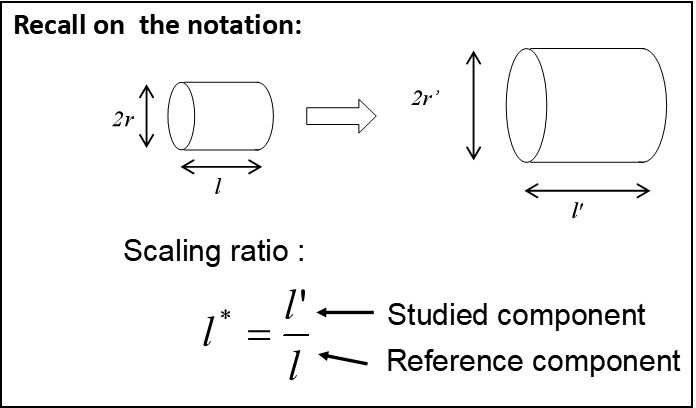
\includegraphics[height=70mm]{Picture1.png}
\end{center}
     \end{discussion} 
 
  
   \begin{question} 
          \begin{center}
	\large{Geometric similarity}
\end{center}
    We assume to have similarity on all geometrical parameters :  $r^* = d^* = …=  l^*$ \\
    \newline
	Give evolutions of areas : 
     \begin{choice}
      \incorrect  $ l^*$
      \incorrect  $ l^{*^2}$ 
      \incorrect $ l^{*^{-2}}$ 
      \correct  $ l^{*^{\frac{1}{2}}}$ 
     \end{choice} 
   \end{question}
     
   \begin{question} 
          \begin{center}
	\large{Geometric similarity}
\end{center}
    We assume to have similarity on all geometrical parameters :  $r^* = d^* = …=  l^*$ \\
    \newline
	Give evolutions of volumes : 
     \begin{choice}
      \incorrect  $ l^*$
      \incorrect  $ l^{*^2}$ 
      \incorrect  $ l^{*^3}$ 
      \incorrect $ l^{*^{-3}}$ 
      \correct  $ l^{*^{\frac{1}{3}}}$ 
     \end{choice} 
   \end{question}
   
   \begin{question} 
          \begin{center}
	\large{Geometric similarity}
\end{center}
     We assume to have similarity on all geometrical parameters :  $r^* = d^* = …=  l^*$ \\
    \newline
	Give evolutions of masses : 
     \begin{choice}
      \incorrect  $ l^*$
      \incorrect  $ l^{*^2}$ 
      \incorrect  $ l^{*^3}$ 
      \incorrect $ l^{*^{-3}}$ 
      \correct  $ l^{*^{\frac{1}{3}}}$ 
     \end{choice} 
   \end{question}
     \begin{question} 
         \begin{center}
	\large{Geometric similarity}
\end{center}
   We assume to have similarity on all geometrical parameters :  $r^* = d^* = …=  l^*$ \\
    \newline
	Give evolutions of intertias : 
     \begin{choice}
      \incorrect  $ l^{*^2}$ 
      \incorrect  $ l^{*^3}$ 
         \incorrect  $ l^{*^4}$
      \incorrect $ l^{*^{5}}$ 
      \correct  $ l^{*^6}$ 
     \end{choice} 
   \end{question}
   
   \begin{question} 
       \begin{center}
	\large{Main design drivers of components}
\end{center}
 Mechanical stress $\sigma$ have a main influence on design of : \\
     \begin{choice}
      \incorrect  Bearings
      \incorrect  Hydraulic jack
         \correct  Brushless motor
     \end{choice} 
   \end{question}
   
    \begin{question} 
    \begin{center}
	\large{Main design drivers of components}
\end{center}
	Temperature $\theta$ and losses have a main influence on design of : \\
     \begin{choice}
      \incorrect  Bearings
      \correct  Hydraulic jack
         \incorrect  Brushless motor
     \end{choice} 
   \end{question}
   
     \begin{question} 
     \begin{center}
	\large{Mechanics: stress}
\end{center}
	\textbf{Recall on the Buckingham theorem} : the theorem states that if there is a physically meaningful equation involving a certain number n of physical variables, then the original equation can be rewritten in terms of a set of p = n - k  dimensionless parameters $\pi_1, \pi_2, ... , \pi_p$ constructed from the original variables where k is the number of independent physical dimensions involved \\
	
	
	Thanks Buckingham theorem, find evolution of stress $\sigma$ with geometrical dimension for a rectangular sample under a load in a three-point bending setup :  
	\begin{minipage}[t]{.8\textwidth}
    \begin{itemize} 
     \item  F is the load (force) at the fracture point (N) 
     \item  L is the length of the support span 
     \item  b is width 
     \item  d is thickness 
     \end{itemize}
      \end{minipage}
\begin{center}
	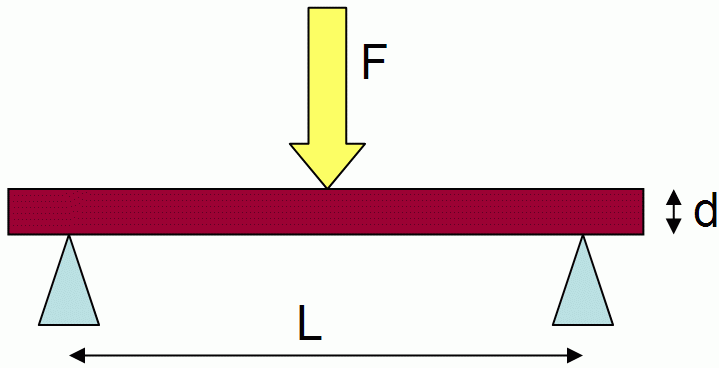
\includegraphics[height=50mm]{Picture2.png}
\end{center}
	
     \begin{choice}
      \incorrect  $\sigma.L.F^{-1} = f(b.L^{-1},d.L^{-1})$
      \correct  $\sigma.L^2.F^{-1} = f(b.L^{-1},d.L^{-1})$
         \incorrect  $\sigma = f(F^{1}.L^{-2},b.L^{-1},d.L^{-1})$
     \end{choice} 
   \end{question}
    \begin{question} 
       \begin{center}
	\large{Mechanics: stress}
\end{center}
Thanks strength theorem of material equation : $\sigma = \frac{3.F.L}{2.b.d^2}$ and geometrical similarity, find scaling laws of stress $\sigma^*$ with geometrical dimension $L^*$ : 

     \begin{choice}
      \incorrect $\sigma^* = F^*.{L^*}^{-2}$
      \correct $\sigma^* = F^*$
         \incorrect  $\sigma^* = F^*.{L^*}^2$
     \end{choice} 
   \end{question}
   
    \begin{question} 
  
        \begin{center}
	\large{Mechanics: stress}
\end{center}
	If $F^*=4$ (force x4) what should be the ratio $L^*$ : 
     \begin{choice}
      \incorrect $L^* = 4$
      \correct $L^* = 2$
         \incorrect  $L^* = 1$
     \end{choice} 
   \end{question}
  
  
     \begin{question} 
        \begin{center}
	\large{Mechanics: stress $\&$ components example}
\end{center}
	Estimate the diameter d of a rod-end with a static load $C_0 = 50 kN $ : 
     \begin{choice}
      \incorrect $d = 5 mm$
      \incorrect  $d = 15 mm$
            \correct  $d = 20 mm$
         \incorrect   $d = 25 mm$
     \end{choice} 
   \end{question}
   
       \begin{question} 
            \begin{center}
	\large{Mechanics: stress $\&$ components example}
\end{center}
	Estimate the mass of a reducer of low speed axe torque 1150 N.m and reduction ratio 10 : 
     \begin{choice}
      \incorrect $m = 5 kg$
      \incorrect  $m = 19,7 kg$
           \correct  $m = 34,5 kg$
         \incorrect   $m = 125,5 kg$
     \end{choice} 
   \end{question}
  
 \begin{question} 
            \begin{center}
	\large{Mechanics: stress $\&$ components example}
\end{center}
	Estimate the linear mass  of the screw shaft characterized by a static load of 5,4 kN : 
     \begin{choice}
      \incorrect $m = 0,12 kg$
      \correct  $m = 0,38 kg$
           \incorrect  $m = 0,64 kg$
         \incorrect   $m = 1,21 kg$
     \end{choice} 
   \end{question}
   
 \begin{question}
      \begin{center}
	\large{Mechanics: stiffness}
\end{center}
	For components with a maximal constant stress, the stress-strain relationship gives : $\sigma = E.\epsilon \Rightarrow   \frac{\Delta l^*}{l^*} = 1$
	
	
	Estimate the torsional backlash of a reducer of low speed axe torque 1150 N.m and reduction ratio 10.

     \begin{choice}
      \correct $\Delta \theta = 3 arcmin$
      \feedback Car $\theta = \frac{\Delta L}{L} = 1$
      \incorrect  $\Delta \theta = 7,6 arcmin$
           \incorrect $\Delta \theta = 1,2 arcmin$
         \incorrect $\Delta \theta = 0,5 arcmin$
     \end{choice} 
   \end{question}
   
   
 \begin{question}
     \begin{center}
	\large{Mechanics: stiffness}
\end{center}

	For components with a maximal constant stress, the stress-strain relationship gives : $\sigma = E.\epsilon \Rightarrow   \frac{\Delta l^*}{l^*} = 1$
	
	
	Estimate the torsional stiffness of a reducer of low speed axe torque 1150 N.m and reduction ratio 10.
     \begin{choice}
      \incorrect $K_t = 530 000 Nm/rad$    
      \correct  $K_t = 1 325 000 Nm/rad$
      \feedback Car $K = \frac{T}{\Delta \theta} = T$
           \incorrect $K_t = 212 000 Nm/rad$
         \incorrect $K_t = 84 000 Nm/rad$
     \end{choice} 
   \end{question}
   
   \begin{question}
    \begin{center}
	\large{Mechanics: resonance modes }
\end{center}

	 Flexural resonance frequency  of plane is given by : $f_r = \alpha_r.\frac{e}{L^2}.\sqrt{\frac{E}{\rho}} $
	 \begin{center}
	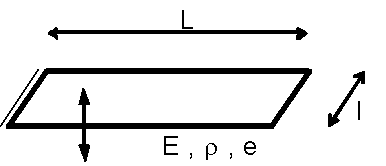
\includegraphics[height=50mm]{Picture3.png}
\end{center}
	In case of geometrical similarity, resonance frequency evolution is given by :


     \begin{choice}
      \incorrect $f_r^* = L^*$    
      \incorrect $f_r^* = {L^*}^{-2}$  
     \incorrect $f_r^* =  {L^*}^{\frac{-1}{2}}$  
      \correct $f_r^* = {L^*}^{-1}$  
     \end{choice} 
     
     
   \end{question}
       
       
        \begin{question}
        
         \begin{center}
	\large{Electrotechnics: induction and heat transfer }
\end{center}
	 For a magnetic circuit including permanent magnets, such as those encountered in brushless motors, the magnetic field can be assumed constant : $B = B_r.\frac{1}{1+\frac{e}{L_m}} \Rightarrow B^* = 1$

	 \begin{center}
	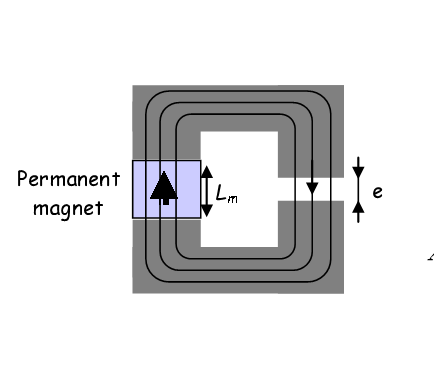
\includegraphics[height=50mm]{Picture4.png}
\end{center}

	In a brushless motor, give the scaling law which links torque $T^*$ to current density $J^*$ and dimensions $L^*$ (geometric similarty assumption) : 



     \begin{choice}
      \incorrect  $T^* = J^*.L^*$    
      \incorrect $T^* = {J^*}^{2}.{L^*}^2$    
     \incorrect $T^* = {J^*}.{L^*}^3$    
      \correct $T^* = {J^*}.{L^*}^4$    
     \end{choice} 
    
   \end{question}
      
  
        \begin{question}
        
	 \begin{center}
	\large{Electrotechnics: induction and heat transfer }
\end{center}
If convective is the main issue for heat transfer of brushless motors, link winding temperature $\theta^*$ to current density $J^*$ and dimensions $L^*$ : 


     \begin{choice}
      \incorrect  $\theta^* = J^*.L^*$    
      \incorrect $\theta^* = {J^*}^{2}.{L^*}^2$    
     \incorrect $\theta^* = {J^*}^2.{L^*}$    
      \correct $\theta^* = {J^*}.{L^*}^2$    
     \end{choice} 
    
   \end{question}

   \begin{question}
        
	 \begin{center}
	\large{Electrotechnics: brushless motors}
\end{center}
The maximum temperature $\theta$  should be constant throughout a range of products, giving :  $\theta^* = 1$  

Estimate the mass of a brushless motor of 8 N.m : 

     \begin{choice}
      \incorrect  $M = 2,1 kg$    
      \correct  $M = 6,8 kg$    
     \incorrect  $M = 4,2 kg$    
      \incorrect  $M = 18 kg$      
     \end{choice} 
    
   \end{question}
   
   \begin{question}
        
	 \begin{center}
	\large{Electrotechnics: brushless motors}
\end{center}

 Estimate the inertia of a brushless motor of 8 N.m : 

     \begin{choice}
      \incorrect  $J = 8.10^{-5} kg.m^2$    
      \incorrect  $J = 22.10^{-5} kg.m^2$    
     \correct  $J = 57.10^{-5} kg.m^2$    
      \incorrect  $J =79.10^{-5} kg.m^2$    
     \end{choice} 
    
   \end{question}

     \end{document}
      